\documentclass[UTF8,a4paper,12pt]{ctexart}
%\usepackage{ctex}
\usepackage{amsmath}
\numberwithin{equation}{section}
\allowdisplaybreaks[4]       %多行公式中换页
\usepackage{array}
\usepackage[font=small,font=bf,labelsep=none]{caption}
\usepackage{amssymb}
\usepackage{tikz}
\usepackage{amsthm}
\usepackage{mathrsfs}
\usepackage{dutchcal}
\usepackage{color}
\usepackage{graphicx}    %插入图片
\usepackage{times}
\usepackage{mathptmx}
\usepackage{fancyhdr} %页眉页脚
\usepackage[backend=biber, style=gb7714-2015]{biblatex}
\usepackage{bicaption}
\usepackage{float}  % 导言区引入
\usepackage[colorlinks=true, linkcolor=blue, urlcolor=blue]{hyperref}
% 文献表条目间的间距
\setlength{\bibitemsep}{0pt}
% 导入参考文献数据库
\addbibresource{main.bib}




\pagestyle{fancy}
\fancyhf{}
\fancyfoot[C]{\thepage}
\usepackage{setspace}
\setlength{\baselineskip}{20pt}
\newcommand*{\circled}[1]{\lower.7ex\hbox{\tikz\draw (0pt, 0pt)%
    circle (.5em) node {\makebox[1em][c]{\small #1}};}}
\usepackage{hyperref}  %目录
\hypersetup{colorlinks=true,linkcolor=black}
\captionsetup[figure][bi-second]{name=Figure} %设置图的英文编号前缀
\captionsetup[table][bi-second]{name=Table} %设置表的英文编号前缀
\numberwithin{equation}{section}%公式按章节编号
\numberwithin{figure}{section}%图表按章节编号
\numberwithin{table}{section}
\renewcommand {\thefigure} {\thesection{}-\arabic{figure}}%设定图片的编号。这样设置的实现效果为图1-1
\renewcommand {\thetable} {\thesection{}-\arabic{figure}}
\usepackage[justification=centering]{caption} %保持居中,防止标题过长导致左对齐
\usepackage{caption}
\captionsetup{font={small},labelsep=quad}%文字5号,之间空一个汉字符位。
\captionsetup[table]{font={bf}} %表格表号与表题加粗
\usepackage{appendix}
\usepackage{tocloft} 
\renewcommand{\cftsecleader}{\cftdotfill{\cftdotsep}} %为目录中section补上引导点
\usepackage{titletoc}
\titlecontents{section}[0pt]{\addvspace{6pt}\filright\bf}%
               {\contentspush{\thecontentslabel \quad }}%
               {}{\titlerule*[8pt]{.}\contentspage}
\makeatletter %双线页眉
\def\headrule{{\if@fancyplain\let\headrulewidth\plainheadrulewidth\fi%
\hrule\@height 1.5pt \@width\headwidth\vskip1.5pt%上面线为1pt粗
\hrule\@height 0.5pt\@width\headwidth  %下面0.5pt粗
\vskip-2\headrulewidth\vskip-1pt}      %两条线的距离1pt
  \vspace{6mm}}     %双线与下面正文之间的垂直间距
\makeatother
% \CTEXsetup[format={\heiti \zihao{3} \bfseries \center}]{section}
% \CTEXsetup[number={第\chinese{section}章}]{section} 

% 自定义章节目录格式
% \ctexset{section={
%   format={\heiti \zihao{3} \bfseries \center},
%   number={第\chinese{section}章}
% }}
\usepackage[explicit]{titlesec}
\titlespacing*{\section}{0pt}{24pt plus .24pt minus .24pt}{18pt plus .0ex}




\begin{document}

\zihao{-4}\songti

\thispagestyle{empty}

\renewcommand{\headrulewidth}{0pt}
\begin{figure}[htb]
\centering % 确保图片和文字居中

\includegraphics[width=1\textwidth]{fig/北京理工大学校徽.png} % 设置图片宽度为页面宽度的80%
\end{figure}

\begin{center}
\songti \zihao{-2} 计算机控制系统课程报告
\end{center}
%该页为中文扉页。无需页眉页脚,纸质论文应装订在右侧
~\\
\begin{center}
\songti \zihao{2} \textbf{正标题 \\ ——副标题}
\end{center}
%中文论文标题,1行或2行,宋体,加粗,二号,居中。论文题目不得超过36个汉字
~\\
~\\
~\\
\begin{center}
\heiti \zihao{3}
\begin{tabular}{l}



\textbf{姓\qquad 名:}XXX\\
\textbf{学\qquad 号:}11202XXXXX\\
\textbf{班\qquad 级:}XXXXXXXX\\ 
\textbf{学\qquad 院:}XXX学院\\ 
\textbf{专\qquad 业:}XX\\ 
\textbf{指导老师:}XXX\\

\end{tabular}
\end{center}
~\\
\begin{center}
\songti \zihao{4} \textbf{\today}
\end{center}

\newpage

\pagenumbering{Roman}

\fancyhead[L]{计算机控制系统课程报告} % 页眉左侧
\fancyhead[R]{摘要} % 页眉右侧

\addcontentsline{toc}{section}{摘\quad 要}
\section*{摘\quad 要}
%摘要:二字间空一格,黑体16磅加粗居中,单倍行距,段前24磅,段后18磅。

\hspace{8mm}本文围绕“XXXXXXXXX”这一主题,分析了XXX。

~\\
\textbf{关键词}:计算机控制系统;数字PID;仿生机器人;脑机接口;抗干扰;智能控制\\
%关键字:宋体12磅,行距20磅,段前段后0磅,关键字之间用逗号隔开,关键词三个字加粗。

\newpage

\fancyhead[L]{计算机控制系统课程报告} % 页眉左侧
\fancyhead[R]{目录} % 页眉右侧

\renewcommand\contentsname{\textbf{目\quad 录}}

\fancypagestyle{plain}{
  \pagestyle{fancy}
}

\begin{center}
{\tableofcontents
}
\end{center}

\newpage

\pagenumbering{arabic}

\fancyhead[LH]{计算机控制系统课程报告}
\fancyhead[RH]{1\quad 绪论}
\section{绪论}

\subsection{研究背景与意义}

\subsection{杭州“六小龙”概况}

图片引用测试\ref{fig:myfig2}:

\begin{figure}[H] % 这里 H 表示 强制放置在当前位置,更改为htbp表示根据需要放置
    \centering
    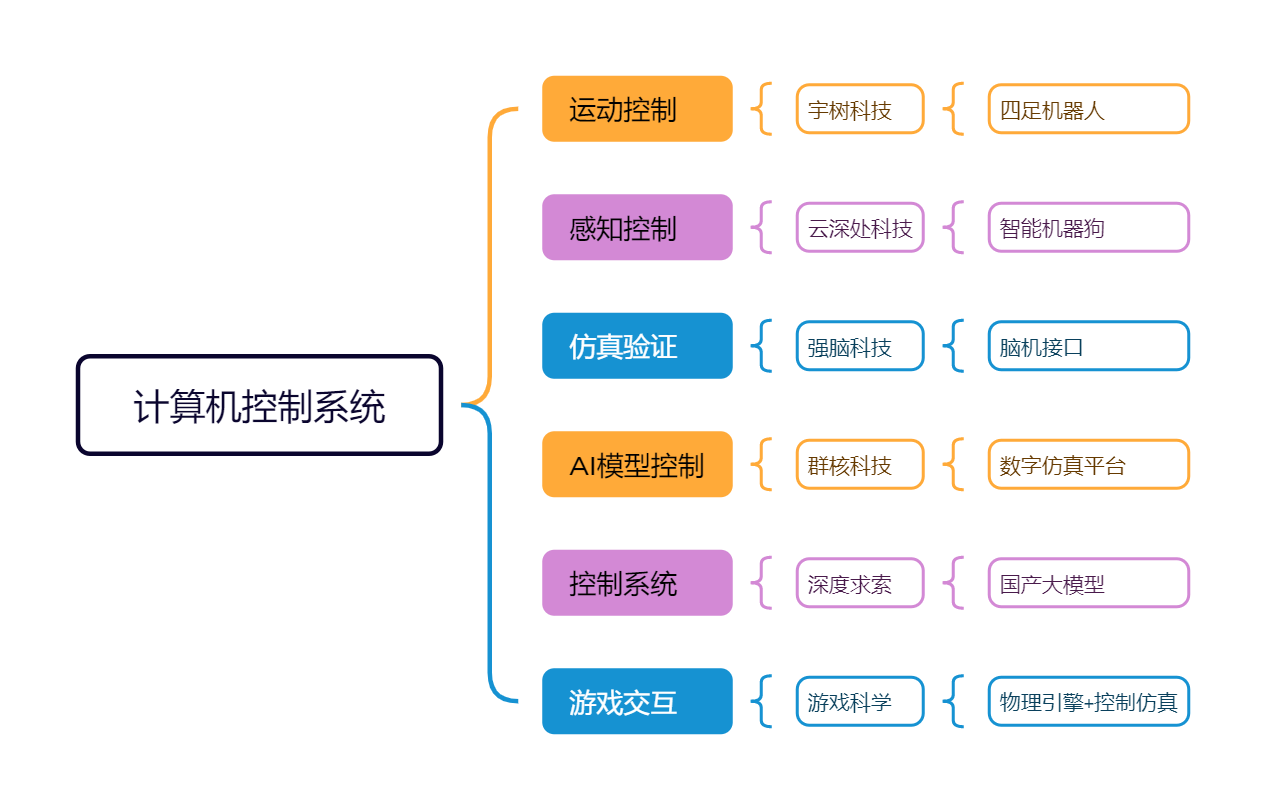
\includegraphics[width=0.8\textwidth]{fig/fig2.png} % 可调整宽度
    \caption{“六小龙”核心技术与计算机控制系统的关系}
    \label{fig:myfig2}
\end{figure}

文献引用示例\cite{ccs}

公式示例\ref{eq:pid-incremental}:
\begin{equation}
    \left\{
    \begin{aligned}
        u(k) &= q_0 e(k) + B(k-1) \\
        B(k) &= u(k) + q_1 e(k-1) + q_2 e(k-2) \\
        q_0 &= K_p \left(1 + \frac{T_s}{T_i} + \frac{T_d}{T_s} \right) \\
        q_1 &= -K_p \left(1 + 2 \cdot \frac{T_d}{T_s} \right) \\
        q_2 &= K_p \cdot \frac{T_d}{T_s}
    \end{aligned}
    \right.
    \label{eq:pid-incremental}
    \end{equation} 

表格示例:
\begin{table}[H]
    \centering
    \caption{高频感应加热的基本参数}
    \begin{tabular}{|c| c|c|c|}
    \hline
    感应频率 &感应发生器功率 & 工件移动速度  &感应圈与零件间隙\\
    (KHz)&($\% \times$80Kw) &(mm/min)  &(mm)\\
    \hline
    250 &88 &5900 &1.65\\
    \hline
    250 &88 &5900 &1.65\\
    \hline
    250 &88 &5900 &1.65\\
    \hline
    250 &88 &5900 &1.65\\
    \hline
    \end{tabular}
\end{table}


\begin{table}
    \centering
    \captionsetup{singlelinecheck=off}
    \caption*{续表} %取消编号
    \begin{tabular}{|c| c|c|c|}
    \hline
    感应频率 &感应发生器功率 & 工件移动速度  &感应圈与零件间隙\\
    (KHz)&($\% \times$80Kw) &(mm/min)  &(mm)\\
    \hline
    250 &88 &5900 &1.65\\
    \hline
    250 &88 &5900 &1.65\\
    \hline
    \end{tabular}
\end{table}
%表格太大需要转页时,需要在续表上方注明“续表”,表头也应重复排出。 % 这里的 tab/tab1.tex 是表格文件的路径

\subsection{报告结构与研究方法}

\newpage

\fancyhead[LH]{计算机控制系统课程报告}
\fancyhead[RH]{2\quad 计算机控制系统核心技术概论}
\section{计算机控制系统核心技术概论}
\subsection{控制系统的基本组成结构}

\subsection{通道接口与系统总线技术}

\subsection{数字控制器设计方法}

\subsection{电磁兼容性设计原则}

\newpage

\fancyhead[LH]{计算机控制系统课程报告}
\fancyhead[RH]{3\quad 仿生机器人系统中的控制技术应用}
\section{仿生机器人系统中的控制技术应用}
\subsection{宇树科技的控制系统架构分析}

\subsubsection{传感器输入与数据采集模块}

\subsubsection{运动控制器与控制算法实现}

\subsubsection{执行器驱动与反馈回路设计}

\subsubsection{系统通信与抗干扰设计}

\subsection{云深处科技的感知融合与控制优化}

\subsubsection{多传感器融合与状态估计}

\subsubsection{路径规划与导航控制器设计}

\subsubsection{执行结构与平台调度}

\subsubsection{系统抗干扰设计与容错机制}

\subsection{控制器设计方法在企业系统中的工程实现}

\newpage

\fancyhead[LH]{计算机控制系统课程报告}
\fancyhead[RH]{4\quad 脑机接口中的计算机控制系统应用}
\section{脑机接口中的计算机控制系统应用}
\subsection{脑机接口技术发展概述}

\subsection{强脑科技的非侵入式脑控系统案例}

\subsection{人机交互系统的闭环反馈控制设计}

\subsection{典型控制系统分析与信号噪声处理对策}

\newpage

\fancyhead[LH]{计算机控制系统课程报告}
\fancyhead[RH]{5\quad 总结与展望}
\section{总结与展望}

\subsection{本文总结}

\subsection{当前存在的挑战与发展瓶颈}

\subsection{对未来技术路线的展望}

\newpage


\fancyhead[LH]{计算机控制系统课程报告}
\fancyhead[RH]{参考文献}


% \addcontentsline{toc}{section}{参\quad 考\quad 文\quad 献}
% \renewcommand\refname{参\quad 考\quad 文\quad 献}

\printbibliography[heading=bibintoc, title={参\quad 考\quad 文\quad 献}]
\newpage

\end{document} 